\documentclass[12pt,a4paper,draft]{article}
\usepackage{amsmath}
\usepackage[numbers]{natbib}
\usepackage{tikz}
\usetikzlibrary{arrows.meta}
\usepackage{booktabs}
\usepackage{microtype}
\usepackage{xurl}

\begin{document}

\title{Optimizing an FPGA-based 3D FDTD Accelerator through HLS}
\author{Tan Jin Hung}
\maketitle

\begin{abstract}
\end{abstract}

\tableofcontents{}

\newpage{}
\section{Introduction}
The current technological era has enabled the use of computers to simulate our complex understanding of the physical world.
However, simulations that accurately mimic real-life phenomena remain computationally intensive for many practical applications.
To manage this complexity, these simulations are often decomposed down into their fundamental physical components.
Among these fundamentals, the simulation of electromagnetic waves remains at the forefront of modern research, with the FDTD method serving as a primary tool for high-fidelity analysis in complex environments \cite{taflove-2005}.

A primary method for simulating electromagnetic waves is the Finite-Difference Time-Domain (FDTD) method \cite{yee-1138693}.
While FDTD is a cornerstone of computational electromagnetics, providing a robust foundation for analysis, it faces significant challenges in 3D space.
Specifically, the iterative nature of the method creates bottlenecks in memory bandwidth and data throughput, often characterized as the 'memory wall' in high-performance computing \cite{nguyen-2022, zohouri-2018}.
As noted by Kong and Su \cite{kong-2016}, the computational demand of the 3D FDTD algorithm increases cubically with the grid resolution, necessitating highly parallel hardware architectures to maintain feasible simulation times.
Traditionally, these simulations have been offloaded to Graphics Processing Units (GPUs).
However, Field-Programmable Gate Arrays (FPGAs) have emerged as a compelling alternative.
FPGAs offer distinct advantages over GPUs, including deterministic latency, superior energy efficiency \cite{nguyen-2022}, and the ability to implement highly customizable memory architectures for parallelism.
Recent research has shown that through customized memory architectures, FPGAs can outperform GPUs in energy-per-update for structured-mesh solvers \cite{kamalakkannan-2023}.

Despite these advantages, FPGAs are traditionally difficult to program using Hardware Description Language (HDLs).
Implementing an FDTD simulation in HDL is tedious and requires the manual design of standard components that are better suited for automation.
High-Level Synthesis (HLS) addresses these challenges by allowing designers to describe complex hardware architectures using high-level languages such as C/C++.
Recent benchmarking has demonstrated that HLS can achieve performance parity with manual RTL design while significantly reducing the development cycle \cite{bai-2023, rodriguez-canal-2023}.

This paper presents an optimized 3D FDTD accelerator designed via HLS, exploring several architectural optimization strategies, including:

\begin{description}
  \item[Spatial Tiling] Maximizing memory bandwidth by utilizing on-chip Block Random Access Memories (BRAMs) to store local stencil and reduce external memory access.
  \item[HLS Directives] Leveraging compiler pragmas to optimize loop pipelining and unrolling, thereby improving the throughput of the kernel.
  \item[Task-Level Parallelism] Decomposing the algorithm into concurrent tasks to increase parallelism.
\end{description}

Through these optimization, we demonstrate that an HLS-driven approach can also produce a high-performance FDTD accelerator, while significantly improving code readability, maintainability, and design iteration speed compared to traditional HDL-based workflows.

\section{Background}
This section establishes the theoretical and technical foundation required to design and implement an FPGA-based 3D FDTD accelerator. 
To provide a complete context for the methodology, the discussion begins with the governing physics of electromagnetic wave propagation through Maxwell’s Equations. 
Subsequently, it details the transition from continuous calculus to a discrete numerical model using Yee’s staggered grid and the resulting leapfrog update equations. 
Finally, the section explores the architectural characteristics of Field-Programmable Gate Arrays (FPGAs) and the High-Level Synthesis (HLS) design flow. 
This hardware background is essential for understanding how algorithmic bottlenecks are addressed through spatial tiling and parallel execution, which are the primary focus of this work.

\subsection{Maxwell's Equation}

The underlying physics governing electromagnetic waves are described by the interaction of electric and magnetic fields, a theory unified by J. C. Maxwell \cite{maxwell-1873}.
Maxwell consolidated the independent laws of Faraday, Amp\`ere, and Gauss, demonstrating that electric and magnetic fields are interdependent. 
While the original theory consisted of 20 equations, it was later refined by O. Heaviside into the modern four-vector representation. 
These equations, representing Gauss's Law, Gauss's Law for Magnetism, Faraday's Law, and Amp\`ere's Law, are given by:

\begin{subequations}
  \label{eq:Maxwell-Heaviside} 
  \begin{align}
    \nabla \cdot \mathbf{D} &= \rho_v \\
    \nabla \cdot \mathbf{B} &= 0 \\
    \nabla \times \mathbf{E} &= -\frac{\partial \mathbf{B}}{\partial t} \\
    \nabla \times \mathbf{H} &= \frac{\partial \mathbf{D}}{\partial t} + \mathbf{J} \\
    \intertext{where the constitutive relations for linear, isotropic media are:}
    \mathbf{D} &= \varepsilon \mathbf{E} \\
    \mathbf{B} &= \mu \mathbf{H} \\
    \mathbf{J} &= \sigma \mathbf{E}
  \end{align}
\end{subequations}

While \eqref{eq:Maxwell-Heaviside} provides a complete description of electromagnetism, it is more practical for numerical wave propagation analysis to substitute the constitutive relations directly into the curl equations. 
By substituting the flux densities ($\mathbf{D}, \mathbf{B}$) and the current density ($\mathbf{J}$) into the curl equations, we obtain the coupled system of first-order partial differential equations:

\begin{subequations}
  \label{eq:Maxwell-lossy}
  \begin{align}
    \nabla \times \mathbf{E} &= - \mu \frac{\partial \mathbf{H}}{\partial t} - \sigma_m \mathbf{H} \\
    \nabla \times \mathbf{H} &= \varepsilon \frac{\partial \mathbf{E}}{\partial t} + \sigma \mathbf{E}
  \end{align}
\end{subequations}

This representation shows explicitly the interaction between the electric ($\mathbf{E}$) and magnetic ($\mathbf{H}$) field intensities, providing the fundamental framework for the FDTD method's time-stepping procedure. 
By rearranging \eqref{eq:Maxwell-lossy} to isolate the temporal derivatives, we obtain the form used for numerical integration:

\begin{subequations}
  \label{eq:Maxwell-temporal}
\begin{align}
  \frac{\partial \mathbf{H}}{\partial t} &= -\frac{1}{\mu} \left( \nabla \times \mathbf{E} + \sigma_m \mathbf{H} \right) \\
  \frac{\partial \mathbf{E}}{\partial t} &= \frac{1}{\varepsilon} \left( \nabla \times \mathbf{H} - \sigma \mathbf{E} \right)
\end{align}
\end{subequations}

\subsection{The FDTD Method}
To solve the coupled system of equations in \eqref{eq:Maxwell-temporal} using a digital computer, the continuous temporal and spatial derivatives must be transformed into a discrete form.
The Finite-Difference Time-Domain (FDTD) method, first proposed by Kane S. Yee in 1966 \cite{yee-1138693}, achieves this by employing central-difference approximations.
This approach maps the electric and magnetic fields onto a discrete staggered grid, allowing the system to be solved iteratively through a "leapfrog" time-stepping procedure.
To ensure the numerical stability of this iterative scheme, the time step must satisfy the Courant-Friedrichs-Lewy (CFL) condition \cite{courant-1967}.

\subsubsection{Yee's Staggered Grid}
To numerically solve Maxwell's equations, the continuous spatial and temporal domains must be discretized.
The FDTD method utilizes the Yee staggered grid, an arrangement where electric ($\mathbf{E}$) and magnetic ($\mathbf{H}$) field components are spatially interleaved within a unit cell, as shown in Figure \ref{fig:YeeCell}, where the $ \mathbf{E} $ field and $ \mathbf{H} $ field are staggered by half a temporal step.

In this configuration, each $\mathbf{E}$ component is located at the center of the edges of a grid cell, while each $\mathbf{H}$ component is positioned at the center of the faces.
The spatial coordinates of the field components within a single Yee cell are summarized in Table \ref{tab:offsets}.

\begin{table}[htbp]
  \label{tab:offsets}
  \centering
  \caption{Spatial offsets for $\mathbf{E}$ and $\mathbf{H}$ field components.}
  \renewcommand{\arraystretch}{1.1}
  \begin{tabular}{l cc}
    \toprule
    \textbf{Axis} & \textbf{Electric Field ($\mathbf{E}$)} & \textbf{Magnetic Field ($\mathbf{H}$)} \\ \midrule
    $x$ & $(i + \frac{1}{2}, j, k)$ & $(i, j + \frac{1}{2}, k + \frac{1}{2})$ \\
    $y$ & $(i, j + \frac{1}{2}, k)$ & $(i + \frac{1}{2}, j, k + \frac{1}{2})$ \\
    $z$ & $(i, j, k + \frac{1}{2})$ & $(i + \frac{1}{2}, j + \frac{1}{2}, k)$ \\ \bottomrule
  \end{tabular}
\end{table}

This spatial staggering ensures that each field component is surrounded by four circulating dual-field components.
This layout provides a natural representation of the curl operators, enabling second-order accurate central-difference approximations.
From a hardware perspective, this arrangement creates a 3D stencil dependency;
updating a single point requires values from its neighbors, which necessitates efficient on-chip memory management to maintain high throughput.

\begin{figure}[htbp]
  \centering
  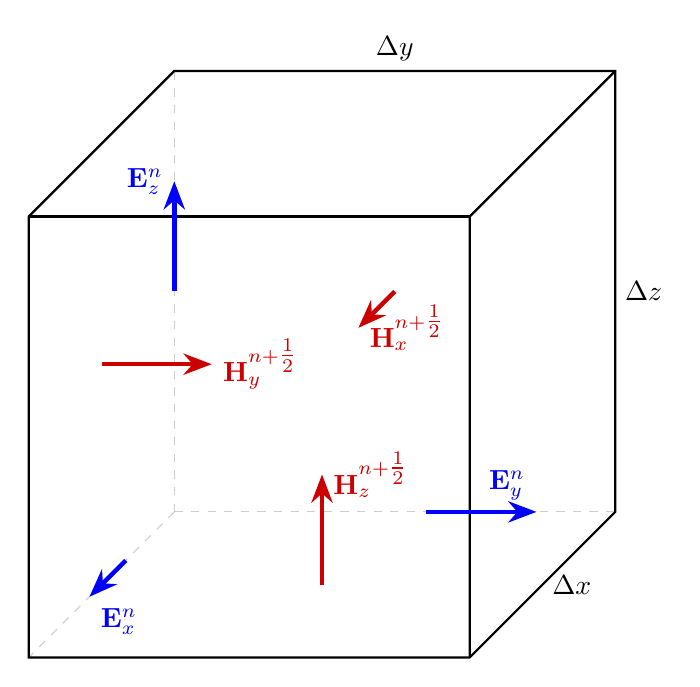
\begin{tikzpicture}[ x={(-0.33cm, -0.33cm)}, y={(1cm,0cm)}, z={(0cm,1cm)}, scale=4, >=Stealth ]
    \def\l{1.4}

    % Grid
    \draw[dashed, gray!40] (0,0,0) -- (0,\l,0);
    \draw[dashed, gray!40] (0,0,0) -- (\l,0,0);
    \draw[dashed, gray!40] (0,0,0) -- (0,0,\l);
    \draw[thick] (\l,0,0) -- (\l,\l,0) -- (0,\l,0) -- (0,\l,\l) -- (0,0,\l) -- (\l,0,\l) -- cycle;
    \draw[thick] (\l,\l,0) -- (\l,\l,\l) -- (0,\l,\l);
    \draw[thick] (\l,0,\l) -- (\l,\l,\l);

    % --- E-fields (Blue) ---
    \draw[->, blue, ultra thick] (\l/3, 0, 0) --++ (\l/4, 0, 0) node[below right] {$\mathbf{E}_x^{ n }$};
    \draw[->, blue, ultra thick] (0, \l/2 + 0.1, 0) --++ (0, \l/4, 0) node[above left] {$\mathbf{E}_y^{ n }$};
    \draw[->, blue, ultra thick] (0, 0, \l/2) --++ (0, 0, \l/4) node[left] {$\mathbf{E}_z^{ n }$};

    % --- H-fields (Red/Orange) ---
    \draw[->, red!80!black, ultra thick] (0, \l/2, \l/2) --++ (\l/4, 0, 0) node[right] {$\mathbf{H}_x^{n+\tfrac{1}{2}}$};
    \draw[->, red!80!black, ultra thick] (\l/2, 0, \l/2) --++ (0, \l/4, 0) node[right] {$\mathbf{H}_y^{n+\tfrac{1}{2}}$};
    \draw[->, red!80!black, ultra thick] (\l/2, \l/2, 0) --++ (0, 0, \l/4) node[right] {$\mathbf{H}_z^{n+\tfrac{1}{2}}$};

    % Labels
    \node[anchor=west] at (\l/2, \l, 0) {$\Delta x$};
    \node[anchor=south] at (0, \l/2, \l) {$\Delta y$};
    \node[anchor=west] at (0, \l, \l/2) {$\Delta z$};
  \end{tikzpicture}
  \caption{Spatial arrangement of electric ($\mathbf{E}$) and magnetic ($\mathbf{H}$) field components. Dimensions $\Delta x, \Delta y, \Delta z$ represent grid increments, and $n$ denotes the temporal step.}
  \label{fig:YeeCell}
\end{figure}

While the Yee grid defines the spatial distribution of the fields, the FDTD method also requires discretization in the temporal domain.
To achieve a stable and accurate simulation, a "leapfrog" time-stepping scheme is employed.
As illustrated in Figure \ref{fig:YeeCell}, the magnetic fields are offset by half a temporal step relative to the electric fields, allowing the interleaved calculation of field updates.

\subsubsection{Temporal Update Equations}
In addition to spatial staggering, the FDTD method employs temporal interleaving, commonly referred to as the "leapfrog" scheme as describe by Taflove \cite{taflove-2005}.
Under this arrangement, the $\mathbf{E}$ components are updated at integer time steps ($n, n+1, \dots$), whereas the $\mathbf{H}$ components are updated at half-integer time steps ($n+1/2, n+3/2, \dots$). 

By applying central-difference approximations to the temporal and spatial derivatives in Maxwell’s Equations, we obtain the explicit update equations.
For a general lossy medium, the update for a single component such as $H_x$ is expressed in Equation \ref{eq:hx_full}:

\begin{equation}
  \label{eq:hx_full}
  \begin{aligned}
    \mathbf{H}_x^{n+1/2}\left[i, j, k\right] &= \left( \frac{1 - \frac{\sigma_m \Delta t}{2\mu}}{1 + \frac{\sigma_m \Delta t}{2\mu}} \right) \mathbf{H}_x^{n-1/2}\left[i, j, k\right] \\
                                            &+ \left( \frac{\frac{\Delta t}{\mu}}{1 + \frac{\sigma_m \Delta t}{2\mu}} \right) \left[ \frac{\mathbf{E}_y^n|_{k+1} - \mathbf{E}_y^n|_k}{\Delta z} - \frac{\mathbf{E}_z^n|_{j+1} - \mathbf{E}_z^n|_j}{\Delta y} \right]
  \end{aligned}
\end{equation}

In the case of a lossless, homogeneous medium such as free space, the conductivities $\sigma$ and $\sigma_m$ are zero.
This reduces the decay coefficients to unity, and the update equations for the full 3D system can be simplified to:

\begin{subequations}
  \label{eq:full_fdtd_vacuum}
  \begin{align}
      \mathbf{H}_x^{n+1/2} &= \mathbf{H}_x^{n-1/2} + \frac{\Delta t}{\mu_0} \left[ \frac{\delta \mathbf{E}_y^n}{\Delta z} - \frac{\delta \mathbf{E}_z^n}{\Delta y} \right] \\
      \mathbf{H}_y^{n+1/2} &= \mathbf{H}_y^{n-1/2} + \frac{\Delta t}{\mu_0} \left[ \frac{\delta \mathbf{E}_z^n}{\Delta x} - \frac{\delta \mathbf{E}_x^n}{\Delta z} \right] \\
      \mathbf{H}_z^{n+1/2} &= \mathbf{H}_z^{n-1/2} + \frac{\Delta t}{\mu_0} \left[ \frac{\delta \mathbf{E}_x^n}{\Delta y} - \frac{\delta \mathbf{E}_y^n}{\Delta x} \right] \\
      \mathbf{E}_x^{n+1} &= \mathbf{E}_x^n + \frac{\Delta t}{\varepsilon_0} \left[ \frac{\delta \mathbf{H}_z^{n+1/2}}{\Delta y} - \frac{\delta \mathbf{H}_y^{n+1/2}}{\Delta z} \right] \\
      \mathbf{E}_y^{n+1} &= \mathbf{E}_y^n + \frac{\Delta t}{\varepsilon_0} \left[ \frac{\delta \mathbf{H}_x^{n+1/2}}{\Delta z} - \frac{\delta \mathbf{H}_z^{n+1/2}}{\Delta x} \right] \\
      \mathbf{E}_z^{n+1} &= \mathbf{E}_z^n + \frac{\Delta t}{\varepsilon_0} \left[ \frac{\delta \mathbf{H}_y^{n+1/2}}{\Delta x} - \frac{\delta \mathbf{H}_x^{n+1/2}}{\Delta y} \right]
  \end{align}
\end{subequations}

where $\delta$ denotes the central-difference operator (e.g., $\delta \mathbf{E}_y^n = \mathbf{E}_y^n|_{k+1} - \mathbf{E}_y^n|_k$, where the index $+1$ refers to the spatial increment along the corresponding axis).

This representation reveals that the field update is a function of the previous state and the surrounding spatial curl, scaled by a material-dependent ratio ($\Delta t/\mu_0$ or $\Delta t/\varepsilon_0$).
These ratios, combined with the grid spacing $\Delta s$, form the basis for the normalized coefficients used in hardware acceleration.

\subsection{Field-Programmable Gate Array (FPGA) Architecture}
While the 3D FDTD algorithm possesses significant inherent symmetry and parallelism, its performance is highly dependent on the ability of the underlying hardware to exploit these features.
Traditionally, Graphics Processing Units (GPUs) have dominated this field due to their massive SIMD (Single Instruction, Multiple Data) parallelism.
However, FPGAs have emerged as a powerful alternative for accelerating computational electromagnetics.

The primary advantage of an FPGA-based design over a GPU lies in its architectural flexibility.
Unlike the fixed memory hierarchy of a GPU, an FPGA allows the designer to implement a fully customized memory architecture, as noted in \cite{kamalakkannan-2023}.
This capability is essential for 3D FDTD, as it enables the creation of application-specific data paths and local memory buffers that can exploit the spatial dependencies of the Yee stencil.
By tailoring the hardware to the algorithm, FPGAs can achieve high throughput with lower power consumption and deterministic latency.
As noted by Zohouri et al. \cite{zohouri-2018}, the advantage of FPGAs in stencil-based high-performance computing lies in their ability to exploit fine-grained parallelism to achieve high performance-per-clock ratios.

To implement the complex update equations defined in Equation \eqref{eq:full_fdtd_vacuum}, the FPGA fabric utilizes several specialized hardware primitives:

\begin{itemize}
  \item \textbf{Configurable Logic Blocks (CLBs):} Consisting of Look-Up Tables (LUTs) and Flip-Flops (FF), these are the fundamental building blocks of the FPGA fabric.
    They implement the "glue logic" and control flow of the system.
    In an HLS-driven design, LUTs are used to build the Finite State Machines (FSMs) that coordinate dataflow between BRAM buffers and DSP slices.
    An increase in available LUTs allows for greater control complexity and more sophisticated optimization strategies.
  
  \item \textbf{Digital Signal Processing (DSP) Slices:} These are dedicated silicon blocks optimized for high-speed arithmetic.
    Each slice typically consists of a pre-defined set of operations, allowing field updates to be performed in a single clock cycle without consuming vast amounts of general-purpose logic.
    An increase in DSP count directly translates to higher throughput, as more field components can be updated in parallel.
    Architecture studies in \cite{kong-2016} demonstrate that the spatial parallelism of FPGAs is uniquely suited to the concurrent field updates of the 3D FDTD grid.
  
  \item \textbf{Block RAM (BRAM):} These represent the on-chip memory resources that distinguish FPGAs from fixed-cache architectures.
    Unlike standard global memory (DRAM), BRAM can be "partitioned" and "reshaped" to provide multiple independent access ports.
    This is a critical feature for stencil computations, where the hardware must fetch several neighboring values simultaneously.
    Increasing BRAM capacity allows larger grid volumes to be stored on-chip, reducing the need for high-latency external memory access.
    Recent methodologies have focused on automatically extracting these memory patterns to reduce the overall FPGA memory footprint for complex stencil codes \cite{szafarczyk-2022}.
\end{itemize}

The performance and scalability of an FPGA-based FDTD accelerator are directly constrained by the availability of these resources.
Since the 3D FDTD algorithm is both computationally and memory-intensive, there is a fundamental trade-off between the simulation volume and the update speed.
A higher count of DSP slices allows for more Processing Elements (PEs) to operate in parallel, while an abundance of BRAM enables the storage of larger grid dimensions on-chip, thereby avoiding the significant latency penalties associated with external DDR memory access.
Consequently, an optimized design must balance the utilization of these resources to maximize the throughput, measured in Millions of cells per second (Mcells/s), while remaining within the physical limits and memory bandwidth constraints of the target device.

\subsection{High-Level Synthesis (HLS)}
While FPGA architectures provide the necessary primitives for acceleration, manual implementation of large-scale projects in low-level Hardware Description Languages (HDLs) is labor-intensive and error-prone.
Many hardware structures, such as memory controllers and nested loop pipelines, follow standard patterns that are better suited for automation than manual coding.
High-Level Synthesis (HLS) addresses these challenges by acting as an abstraction layer that automates the generation of these standard structures \cite{vitis-ug1399-2025}.
Furthermore, HLS allows designers to describe complex projects using high-level languages like C or C++, significantly lowering the barrier of entry compared to RTL design in Verilog or VHDL.

To bridge the gap between algorithmic description and hardware realization, HLS provides several critical optimization directives and data-handling paradigm \cite{vitis-ug1399-2025}:
\begin{itemize}
    \item \textbf{Pipelining (\texttt{\#pragma HLS PIPELINE}):} This is a fundamental optimization for FDTD.
      It enables the concurrent execution of different stages of the update equation.
      By pipelining the inner loops, the hardware can begin a new field update before the previous one has completed, with the primary objective of achieving an Initiation Interval (II) of 1.

    \item \textbf{Memory Partitioning (\texttt{\#pragma HLS ARRAY\_PARTITION}):} Standard BRAM is limited by its physical port count (typically two).
      Since 3D FDTD stencils require multiple simultaneous operands, HLS allows for the "partitioning" of these arrays into smaller, independent memory banks.
      This provides the parallel access ports necessary to feed the DSP update engines without stalling the pipeline, a technique widely utilized to overcome the memory bottlenecks of structured-mesh solvers \cite{kamalakkannan-2023, szafarczyk-2022}.

    \item \textbf{Task-Level Parallelism (\texttt{\#pragma HLS DATAFLOW}):} This directive enables the execution of functions in a producer-consumer pattern.
      In the context of this work, it allows the electric and magnetic field update functions to operate concurrently, overlapping their execution to maximize the utilization of the FPGA’s spatial resources.

    \item \textbf{Streaming Interfaces (\texttt{hls::stream} or \texttt{hls::stream\_of\_blocks}):} Beyond standard memory-mapped access, HLS supports a streaming data paradigm through built-in libraries (\texttt{hls\_streamofblocks.h} or \texttt{hls\_stream.h}).
      Using FIFO (First-In-First-Out) buffers, data can be passed point-to-point between hardware modules without the overhead of global memory addressing.
      In 3D FDTD, streaming is essential for moving planes of data through the update engine, minimizing latency and enabling the high-throughput "Stream of Blocks" architecture\cite{so-2018}.
\end{itemize}

By utilizing these directives, HLS enables a "stepwise refinement" design process.
A designer can begin with a baseline software implementation and iteratively apply hardware constraints to transform a sequential C-program into a high-performance, parallelized 3D FDTD accelerator.
As shown in automation frameworks such as SASA \cite{tian-sasa-2023}, overlapping computation and communication optimizations are critical for scaling FDTD accelerators to handle massive data volume of 3D electromagnetic simulations.

\section{Methodology}

\subsection{Baseline Implementation}
\subsection{Domain Decomposition}
\subsection{Memory Subsystem Optimization}
\subsection{Advanced Throughput Optimization}

\section{Evaluation}
\subsection{Environments}
\subsection{Results}

\section{Discussion}

\section{Conclusion}

\clearpage{}
\sloppy
\bibliographystyle{IEEEtranN}
\bibliography{references}
\end{document}
